\documentclass[11pt,a4paper]{ctexart}
\usepackage{ctex}
\usepackage{graphicx}
\usepackage{epstopdf}
\usepackage{xcolor}
\usepackage{amssymb}
\usepackage{amsmath}
\usepackage{amsfonts}
\usepackage{subfigure}
\usepackage{float}
\usepackage{cases}
\usepackage{cmap}
\usepackage{stfloats}
\usepackage{booktabs}
%\usepackage{cite}
\usepackage{ulem}
\usepackage{multirow}
\usepackage{titlesec}
\setcounter{table}{0}
\usepackage[CJKbookmarks,breaklinks=true]{hyperref}
\usepackage{cleveref}
\pagestyle{plain}
\topmargin=-1.5cm
\oddsidemargin=-0.55cm \evensidemargin=0pt
\textwidth=17cm
\textheight=25cm
\newtheorem{theorem}{定理}[section]
\newtheorem{definition}{定义}[section]
\usepackage{ulem} 
\usepackage[square, comma, sort&compress, numbers]{natbib}
\newcommand\dx{\,\mathrm{d}x}% 定义微分符号dx
\newcommand\dt{\,\mathrm{d}t}
\newcommand\dy{\,\mathrm{d}y}
\newcommand\dd{\,\mathrm{d}}
\newcommand\dint{\displaystyle \int} 
\newcommand\myciteup[1]{{\setcitestyle{square,super}\cite{#1}}}
\usepackage{caption}
\captionsetup{labelformat=default,labelsep=space} %去除冒号

% 参考文献
%\bibliographystyle{unsrt}
%\usepackage{gbt7714}
% 参考文献输出方式，numerical为按照出现顺序，authoryear为按照作者姓名和年份
%\bibliographystyle{gbt7714-numerical}

\begin{document}
\title{怪波，呼吸子和耦合薛定谔方程的亮-暗-怪解（郭柏灵，凌黎明）}
\author{第七小组-黄伟宁}
\maketitle

\begin{abstract}
	本文通过Darboux变换构造了耦合非线性薛定谔方程具体的怪波解，呼吸子（孤立子）解，和怪-亮-暗解。
\end{abstract}

\textbf{关键词}：耦合薛定谔方程，Darboux变换，呼吸子解，怪波解，怪-亮-暗解

\section{引言}

耦合薛定谔方程（CNLS/NLS）是一个重要的模型，尤其是在非线性光学，生物物理学，零度条件下的多模块Bose-Einstein凝聚,经济学和海洋学。然而，选定特殊的参数之后方程会变得可积（Manakov模型）。另外，Manakov模型也出现在一个对光折变晶体的Kerr型近似中。因此，该方程可以具体地描述一些物理现象。已经有很多关于这类系统的研究。

在这篇通信中，我们考虑一个可积的耦合薛定谔方程
\begin{align*}
	 & iq_{1t} +q_{1xx} +2(|q_{1} |^{2}+|q_{2} |^{2})q_{1} =0,\tag{1a}   \\
	 & iq_{2t} +q_{2xx} +2(|q_{1} |^{2} +|q_{2} |^{2} )q_{2} =0.\tag{1b}
\end{align*}
Manakov证明了这个系统的可积性。最近，在非线性科学领域怪波现象的研究热度很高。怪波是在特定条件下会在海洋中出现的强小波。这些波的高度可以达到一般波高的两倍、三倍，甚至更多倍。怪波也被熟知为奇异波，怪兽波，杀手波，巨波或者极端波。Peregrine在1983年给出了非线性Schr\"{o}dinger方程的一阶有理解。NLS方程的怪波是通过Darboux变换导出的。最近，我们通过Darboux-Liouville变换构造了一些更一般的怪波解。众所周知，已经有很多关于非线性Schr\"{o}dinger方程的怪波的研究结果。但是，极尽我们所知，尚没有关于耦合薛定谔方程的具体怪波解的报告。与此同时我们也得到了新的呼吸子解和亮-暗-怪解作为副产品。

Darboux变换是构造可积系统一些有趣的解的有力工具（孤立子，移位子，怪波解）。我们工作的目标是用Darboux变换去构造怪波解，呼吸子和亮-暗-怪解。这些特别的解可能可以在一些物理现象比如BEC或非线性光学的研究中发挥重要作用。

\section{求解过程}

第一步，我们通过Darboux变换构造怪波解。系统(1)有如下的Lax对
\begin{align*}
	 & \Phi_{x} =U\Phi=[i\zeta U_{1} +U_{0} ]\Phi,\tag{2a}                                                \\
	 & \Phi_{t} =V\Phi=[3i\zeta^{2} U_{1} +3\zeta U_{0} +i\sigma_{3} (U_{0,x} -U_{0} ^{2} )]\Phi,\tag{2b}
\end{align*}
其中
$$
	U_{0} =\begin{pmatrix}
		0           & q_{1} & q_{2} \\
		-q_{1} ^{*} & 0     & 0     \\
		-q_{2} ^{*} & 0     & 0
	\end{pmatrix},
$$
$ U_{1}   =\text{diag}\{-2,1,1\}, \sigma_{3}=\text{diag}\{1,-1,1\}$,并且$ \Phi $ 是特征函数构成的矩阵，$ \zeta $ 是谱参数。Lax对(2)的相容性条件给出了CNLS(1)。众所周知(2)的Darboux变换是
\begin{align*}
	T=\zeta I-[\zeta_{1} ^{*} -(\zeta_{1} ^{*} -\zeta_{1} )P_{1} ],\quad P_{1} =\frac{\Phi_{1} \Phi_{1} ^{\dagger} }{\Phi_{1} ^{\dagger} \Phi_{1} },\tag{3}
\end{align*}
其中$ \Phi_{1} =\Phi(x,t,\zeta_{1} )(m_{1} ,m_{2},m_{3})^{T} $，$ m_{1} ,m_{2} ,m_{3}  $ 是常数，$ I $ 是三阶单位阵且$ \Phi(x,t,\zeta_{1} ) $ 是Lax对方程在$ \zeta=\zeta_{1} ,q_{i} =q_{i} [0](i=1,2) $时的基本解组。然后是域之间的变换
\begin{align*}
	q_{1} [1]=q_{1} [0]+6\text{Im}(\zeta_{1} )\frac{\phi_{1} \phi_{2} ^{*} }{|\phi_{1} |^{2} +|\phi_{2} |^{2} +|\phi_{3} |^{2} }, \\
	q_{2} [1]=q_{2} [0]+6\text{Im}(\zeta_{1} )\frac{\phi_{1} \phi_{3} ^{*} }{|\phi_{1} |^{2} +|\phi_{2} |^{2} +|\phi_{3} |^{2} },\tag{4}
\end{align*}
其中$ (\phi_{1} ,\phi_{2} ,\phi_{3} )^{T} =\Phi_{1} $。

我们从种子解——平面波解开始。记
\begin{align*}
	q_{1} [0]=c_{1} \exp[i\theta_{1}],\quad q_{2} [0]=c_{2} \exp[i\theta_{2} ],\tag{5}
\end{align*}
其中$ \theta_{i} =d_{i}x+(2c_{1} ^{2} +2c_{2} ^{2} -d_{i} ^{2} )t  $ ，$ c_{i}  $ 和$ d_{i}(i=1,2)  $ 是任意常数。然而，Lax对方程是变系数微分方程，我们不能直接求解。幸运的是，我们可以通过一个巧妙的变换把这个系统变成一个常系数微分方程组。接下来，我们给出Lax对方程(2)在$ q_{1} =q_{1} [0] $ 和$ q_{2} =q_{2} [0] $ 	时候的变换。我们可以得到
\begin{align*}
	 & \Psi_{x} =(MUM^{-1} +M_{x} M^{-1} )	\Psi=U_{1} \Psi,       \\
	 & \Psi_{t} =(MVM^{-1} +M_{t} M^{-1} )\Psi=V_{1} \Psi,\tag{6}
\end{align*}
其中$ \Psi=M\Phi,M=\text{diag}\{\exp[-\frac{i}{3}(\theta_{1} +\theta_{2} )],\exp[\frac{i}{3}(2\theta_{1} -\theta_{2} )],\exp[\frac{i}{3}(2\theta_{2} -\theta_{1} )]\} $ 。简单计算之后，我们有
\begin{align*}
	U_{1} =\begin{pmatrix}
		       \chi_{11} & c_{1}     & c_{2}     \\
		       -c_{1}    & \chi_{22} & 0         \\
		       -c_{2}    & 0         & \chi_{33}
	       \end{pmatrix},                                      \\
	V_{1} =iU_{1} ^{2} -[\frac{2}{3}(d_{1} +d_{2} )-2\zeta_{1} ]U_{1} +mI,\tag{7} \\
	\chi_{11} =-2i\zeta_{1} -\frac{i}{3}(d_{1} +d_{2} ),                          \\
	\chi_{22} =I\zeta_{1} +\frac{i}{3}(2d_{1} -d_{2} ),                           \\
	\chi_{33} =i\zeta_{1} +\frac{i}{3}(2d_{2} -d_{1} ),
\end{align*}
其中$ m=2i\zeta_{1} ^{2} +\frac{2i}{3}(c_{1} ^{2} +c_{2} ^{2} )+\frac{2i}{9}(d_{1} ^{2} -d_{1} d_{2} +d_{2} ^{2} )+\frac{2i\zeta_{1} }{3}(d_{1} +d_{2} ) $。在参考文献中有人考虑了$ U_{1}  $ 的特征多项式有一个单根和一个二重根时候的解。事实上，$ U_{1}  $ 的特征多项式可以有一个三重根。我们的工作是寻找在这种特殊情况下方程的解。方程(6)是常系数微分方程组。为了寻找有理解，我们选择满足$ \alpha=d_{2} +3e_{1} ,e_{1} =\text{Re}(\zeta_{1} ),d_{1} =d_{2} -2\alpha,c_{1} =\pm 2\alpha,c_{2} =\pm 2\alpha,\text{Im}(\zeta_{1} )=\pm\sqrt{3}\alpha $，$ d_{2}  $和$ \text{Re}(\zeta_{1} ) $ 是任意实数。矩阵$ U_{1}  $ 不能对角化，只能进行Jordan标准型分解。因此Lax对方程(2)在$ \zeta=\zeta_{1} ,q_{i} =q_{i} [0](i=1,2) $ 的基本解组矩阵是$ \Phi(x,t,\zeta_{1} )=M^{-1} \Theta $，
\begin{gather*}
	\Theta=\begin{pmatrix}
		\varpi_{11} & 4\alpha^{2} \gamma+2\sqrt{3}\alpha      & 4\alpha                   \\
		\varpi_{12} & -2\alpha^{2} (\sqrt{3}-i)\gamma-2\alpha & -2\alpha^{2} (\sqrt{3}-i) \\
		\varpi_{13} & -2\alpha^{2} (\sqrt{3}+i)\gamma-2\alpha & -2\alpha^{2} (\sqrt{3}+i)
	\end{pmatrix}, \\
	\varpi_{11} =4\alpha^{2} (\gamma^{2} +2it)+4\sqrt{3}\alpha\gamma+2,                      \\
	\varpi_{12} =-2(\sqrt{3}-i)\alpha^{2} (\gamma^{2} +2it)-4\alpha\gamma,\\
	\varpi_{13} =-2(\sqrt{3}+i)\alpha^{2} (\gamma^{2} +2it)-4\alpha\gamma,
\end{gather*}
其中$ \gamma=x+2\sqrt{3}\beta it $，且$ \beta=\alpha-i\sqrt{3}e_{1}  $。接下来，我们用Darboux变换(4)导出CNLS(1)的有理解。

\section{怪波解}

（1）怪波解1。选择参数$ m_{1} =0,m_{2} =1,m_{3} =0 $，我们通过公式(4)可以得到怪波解1
\begin{align*}
	q_{1} [1]=\alpha[-1-i\sqrt{3}+\frac{-6\delta\alpha\sqrt{3}-36t\alpha^{2}\sqrt{3}-3+i(36\alpha^{2} t+6\delta\alpha+5\sqrt{3})}{12\alpha^{2} \delta^{2} +8\delta\alpha\sqrt{3}+144t^{2} \alpha^{4} +5}]\cdot\exp[i\theta_{1} ], \\
	q_{2} [1]=\alpha[-1+i\sqrt{3}+\frac{-6\delta\alpha\sqrt{3}+36t\alpha^{2} \sqrt{3}-3+i(36\alpha^{2} t-6\delta\alpha-5\sqrt{3})}{12\alpha^{2} \delta^{2} +8\delta\alpha\sqrt{3}+144\alpha^{4} t^{2} +5}]\cdot\exp[i\theta_{2} ],\tag{8}
\end{align*}
其中$ \delta=x+6e_{1} t $ 。这种类型的怪波解跟非线性薛定谔方程的一阶怪波解是相似的。

（2）怪波解2。选择参数$ m_{1} =1,m_{2} =0,m_{3} =0 $ ，我们可以通过公式得到怪波解2
\begin{align*}
	q_{1}[1]=\alpha[-1-i\sqrt{3}+\frac{G_{1} +iH_{1} }{D}]\exp[i\theta_{1} ], \\
	q_{2} [1]=\alpha[-1+i\sqrt{3}+\frac{G_{2} +iH_{2} }{D}]\exp[i\theta_{2} ],\tag{9}
\end{align*}
其中
\begin{align*}
	D     & =1728\alpha^{8} t^{4} +288\alpha^{6} \delta^{2} t^{2} +384\sqrt{3}\alpha^{5} \delta t^{2} +12\alpha^{4} \delta^{4} +432\alpha^{4} t^{2} +16\sqrt{3}\alpha^{3} \delta^{3} +24\alpha^{2} \delta^{2} +4\sqrt{3}\alpha\delta+1,                \\
	G_{1} & =-864\sqrt{3}\alpha^{6} t^{3} -144\sqrt{3}\alpha^{5} \delta t^{2} -72\sqrt{3}\alpha^{4} \delta^{2} t-216\alpha^{4} t^{2} -12\sqrt{3}\alpha^{3} \delta^{3} +144\alpha^{3} \delta t-18\alpha^{2} \delta^{2} +12\sqrt{3}\alpha^{2} t+3,       \\
	G_{2} & =+864\alpha^{6} t^{3} -144\alpha^{5} \delta t^{2} +72\sqrt{3}\alpha^{4} \delta^{2} t-216\alpha^{4} t^{2} -12\sqrt{3}\alpha^{3} \delta^{3} +144\alpha^{3} \delta t-18\alpha^{2} \delta^{2} +12\sqrt{3}\alpha^{2} t+3,                       \\
	H_{1} & =+864\alpha^{6}t^{3} +144\alpha^{5} \delta t^{2} +72\alpha^{4} \delta^{2} t+312\sqrt{3}\alpha^{4} t^{2} +12\alpha^{3} \delta^{3} +96\sqrt{3}\alpha^{3} \delta t+18\sqrt{3}\alpha^{2} \delta^{2} +108\alpha^{2} t+12\alpha\delta+\sqrt{3},  \\
	H_{2} & =+864\alpha^{6} t^{3} -144\alpha^{5} \delta t^{2} +72\alpha^{4} \delta^{2} t-312\sqrt{3}\alpha^{4} t^{2} -12\alpha^{3} \delta^{3} +96\sqrt{3}\alpha^{3} \delta t-18\sqrt{3}\alpha^{2} \delta^{2} +108\alpha^{2} t-12\alpha\delta-\sqrt{3}.
\end{align*}
选择合适的参数，$ |q_{1} [1]|^{2} $和$ |q_{2} [2]|^{2}  $ 的图像如图1所示。在NLS的怪波下他们有不同的行为。事实上我们可以把三个向量解组合起来去得到一个新的怪波，但是我们不能得到除了以上两种类型以外别的类型的解。通过对称分析可以发现我们得到的怪波跟参考文献出现过的是不一样的，实际上二者并没有本质区别，他们只是NLS的海拔不同的怪波解而已。
\begin{figure}
	\centering
	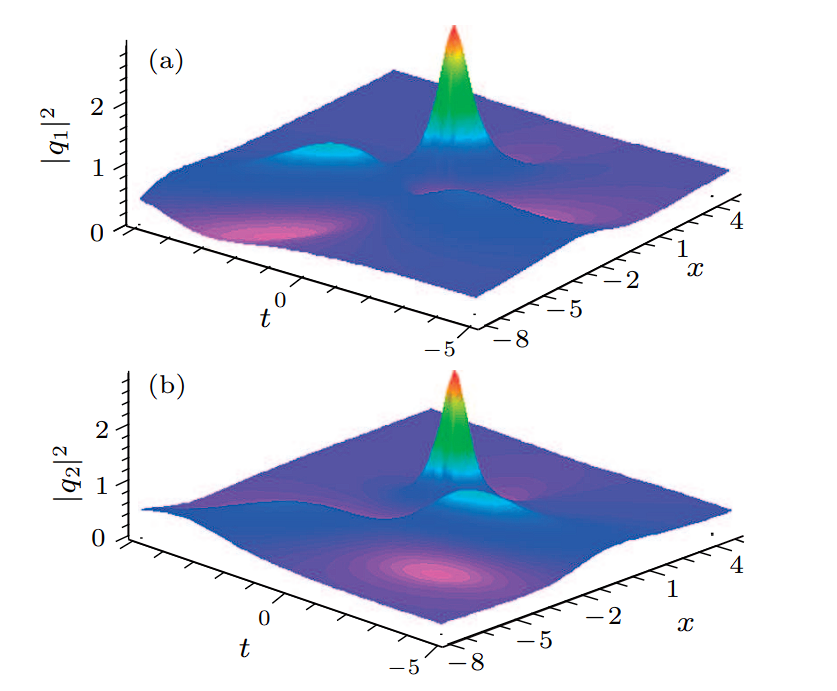
\includegraphics[scale=0.3]{fig1.png}
	\caption{$ |q_{1} |^{2}  $ 和$ |q_{2} |^{2}  $ 在参数$ e_{1} =\frac{1}{10},d_{1} =0 $ 时除了海拔以外的不同行为}
\end{figure}
\begin{figure}
	\centering
	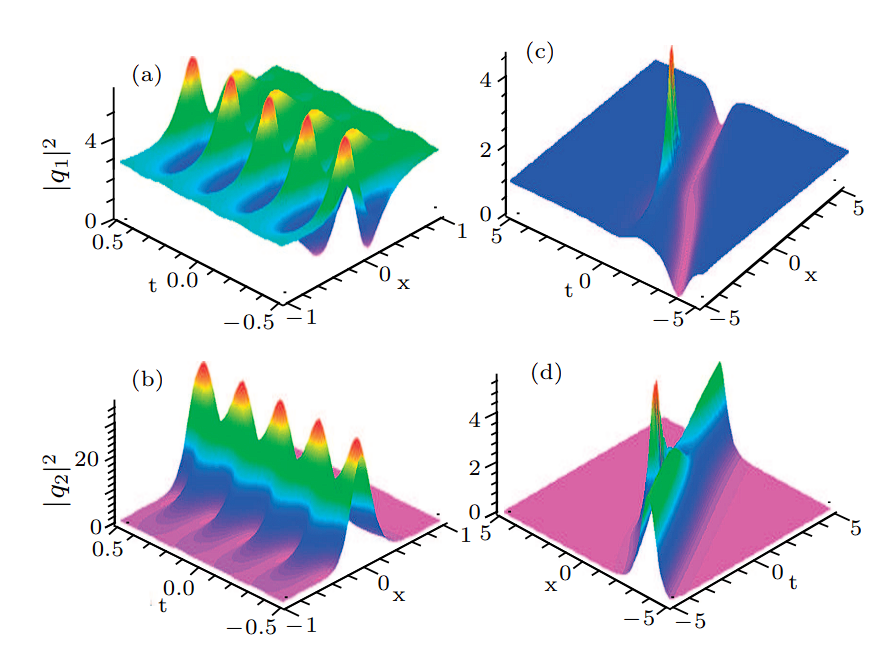
\includegraphics[scale=0.3]{fig2.png}
	\caption{图(a)和(b)取的参数是$ c=-2,d=0,\zeta_{1} =2i,\lambda_{1} =1-\sqrt{5},\tau_{1} =\tau_{2} =\kappa_{1} =\kappa_{2} =0$；然后亮-暗-怪解(c)和(d)取的参数是$ c=d=1,c_{1} =c_{2} =c_{3} =1 $ 。 }
\end{figure}

我们可以轻松地得到如下关于怪波解的关系式，
\begin{align*}
	\int_{-\infty} ^{\infty} (|q_{1} [1]|^{2} -4\alpha^{2} )\dx=0, \\
	\int_{-\infty} ^{\infty} (|q_{2} [1]|^{2} -4\alpha^{2} )\dx=0.\tag{10}
\end{align*}
这意味着$ |q_{1} [1] |^{2} $和$ |q_{2} [1] |^{2} $在如上背景之下有同等地位。

\section{呼吸子解，亮-暗解和亮-暗-怪解}

更进一步地，我们考虑了另外一种有趣的情况：一个是零解而另外一个是平面波解。有趣的是，我们可以通过这种情况得到呼吸子解、一个亮-暗解和一个亮-暗-怪解。接下来，我们从种子解$ q_{1} [0]=c\exp[i\theta],q_{2} [0]=0 $ 开始，其中$ \theta=dx+(2c^{2} -d^{2} )t $ 。类似地，我们取$ M=\text{diag}\{1,\exp[i\theta],1\} $。然后我们可以得到如下结果
\begin{align*}
	 & U_{1} = \begin{pmatrix}
		           -2i\zeta_{1} & c              & 0          \\
		           -c           & i\zeta_{1} +id & 0          \\
		           0            & 0              & i\zeta_{1}
	           \end{pmatrix},                                            \\
	 & V_{1} =iU_{1} ^{2} +2\zeta_{1} U_{1} +2i(\zeta_{1} ^{2} +c^{2}) -\text{diag}\{0,0,2ic^{2} \}.
\end{align*}
$ U_{1}  $ 的特征方程是$ (\lambda-i\zeta_{1} )[(\lambda+2i\zeta_{1} )(\lambda-i\zeta_{1} -id)+c^{2} ]=0 $。然后我们可以根据解的不同性态把特征方程分为两类。

情况1：单根。假设$ U_{1}  $ 的特征方程有三个不同的根，把它们记作$$ i\zeta_{1} ,\lambda_{1} =\frac{i}{2}[-\zeta_{1} +d+\sqrt{9\zeta_{1} ^{2} +6\zeta_{1} d+d^{2} +4c^{2} }],\lambda_{2} =i(d-\zeta_{1} )-\lambda_{1}  $$最后，我们可以得到Lax对方程的基本解组矩阵$ \Phi(x,t,\zeta_{1} )=M^{-1} Q\Omega $ ，
\begin{gather*}
	Q=\begin{pmatrix}
		0 & c                        & \lambda_{1} +2i\zeta_{1} \\
		0 & \lambda_{1} +2i\zeta_{1} & c                        \\
		1 & 0                        & 0
	\end{pmatrix},\\
	\Omega=\begin{pmatrix}
		e^{i\zeta_{1} x+3i\zeta_{1} ^{2} t} & 0           & 0           \\
		0                                   & \kappa_{22} & 0           \\
		0                                   & 0           & \kappa_{33}
	\end{pmatrix},\\
	\kappa_{22} =\exp\{\lambda_{1} x+[i\lambda_{1} ^{2} +2\zeta_{1} \lambda_{1} +2i(\zeta_{1} ^{2} +c^{2} )]t\},\\
	\kappa_{33} =\exp\{\lambda_{2} x+[i\lambda_{2} ^{2} +2\zeta_{1} \lambda_{2} +2i(\zeta_{1} ^{2} +c^{2} ) ]t\}.
\end{gather*}

把代入公式(4)的解替换掉并且取参数$ m_{1} =1,m_{2} =e^{\tau_{1} +i\kappa_{1} } ,m_{3} =e^{\tau_{2} +i\kappa_{2} } $（$ \tau_{i} ,\kappa_{i} (i=1,2) $是任意实数 ），我们可以得到CNLS方程的呼吸子解。这种类型的解是周期函数或者准周期函数。通过取合适的参数，图2(a)和图2(b)展现了解$ q_{1} [1] $ 和$ q_{2} [1] $ 的动态行为。当$ \text{Re}(\zeta_{1} )=\text{Im}(\lambda_{1} )=d=0 $，这个解是一个时间周期函数并且周期是$ 2\pi/|d^{2} -\text{Im}(\zeta_{1} ^{2} )| $。

情况2：重根。假设$ \zeta_{1} =-\frac{1}{3}(d+2ic) $，$ U_{1}  $ 的特征方程会有一个二重根。随即可以得到Lax对方程在$ \zeta_{1} =-\frac{1}{3}(d+2ic) $ 的基本解组矩阵是$ \Phi(x,t,\zeta_{1} )=M^{-1}Q\Omega    $ ，
\begin{gather*}
	Q=\begin{pmatrix}
		0 & -c & 1 \\
		0 & -c & 0 \\
		1 & 0  & 0
	\end{pmatrix},\\
	\Omega=\begin{pmatrix}
		0               & 0                           & \exp(\eta_{1} ) \\
		\exp(\eta_{2} ) & [x-2(d+ic)t]\exp(\eta_{2} ) & 0               \\
		0               & \exp(\eta_{2} )             & 0
	\end{pmatrix},\\
	\eta_{1} =\frac{1}{3}(2c-id)x+\frac{1}{3}[-4cd+i(d^{2} -4c^{2} )]t,\\
	\eta_{2} =\frac{1}{3}(-c+2id)x+\frac{1}{3}[2cd+i(5c^{2} -2d^{2} )]t.
\end{gather*}
又一次替换代入公式(4)的解，我们可以得到亮-暗解和亮-暗-怪解。如果我们取参数$ c_{3} =0 $ ,随即可以得到$ q_{1} [1] $ 是NLS方程的怪波解并且$ q_{2} [1]=0 $ 。接下来，我们考虑另外两种非平凡的情况。

情况2（1）：取参数$ m_{1} =1,m_{2} =0 ,m_{3} =a_{3} +b_{3} i $ ,我们可以得到亮-暗孤立子，
\begin{gather*}
	q_{1} [1]=c\tanh(\frac{3}{2}\eta_{1r} +\mu)\exp(i\theta),\\
	q_{2} [1]=-4c^{2} (a_{3} +ib_{3} )\text{sech}(\frac{3}{2}\eta_{1r} +\mu)\cdot\exp[i(dx+(3c^{2} -d^{2} )t)],
\end{gather*}
其中$ \eta_{1r} =\frac{2c}{3}(x-2dt) $且$ \mu=\frac{1}{2}\ln(\frac{a_{3} ^{2} +b_{3} ^{2} }{2c^{2} }) $ 。有趣的是我们可以在聚焦行为和异常分散纤维中得到亮-暗孤立子解。

情况2（2）：取参数$ m_{1} =a_{1} +b_{1} i,m_{2} =1,m_{3} =a_{3} +b_{3} i $ 我们有
\begin{align*}
	q_{1} [1]= & c\{1-4[a_{1} ^{2} +\alpha_{2} ^{2} -\alpha_{1} +i\alpha_{2} ]\exp(-\eta_{1r} )\cdot\{[2(\alpha_{1} ^{2} +\alpha_{2} ^{2} )-2\alpha_{1} +1]\exp(-\eta_{1r} ) \\
	           & +(a_{3} ^{2} +b_{3} ^{2} )\exp(2\eta_{1r} )\}^{-1}\}\exp(i\theta),                                                                                          \\
	q_{2} [1]= & -4c[a_{3} (\alpha_{1} -1)-b_{3} \alpha_{2} +i[a_{3} \alpha_{2} +b_{3} (\alpha_{1} -1)]]\cdot\exp[\frac{1}{2}\eta_{1r} +i(dx+(3c^{2} -d^{2} )t)]             \\
	           & \cdot\{[2(\alpha_{1} ^{2} +\alpha_{2} ^{2} )-2\alpha_{1} +1]\exp(-\eta_{1r} )+(a_{3} ^{2} +b_{3} ^{2} )\exp(2\eta_{1r} )\}^{-1} ,
\end{align*}
其中$ \alpha_{1} =a_{1} c+c(x-2dt),\alpha_{2} =b_{1} c-2c^{2} t $。我们选择合适的参数并用图片展示了这种类型的解（图2(c)和图2(d)）。这种解表现得像怪波解和亮-暗孤立子解的非线性叠加。

%\cleardoublepage
%\phantomsection
%\addcontentsline{toc}{chapter}{参考文献}
%\nocite{*} %排版所有包括未引用的文献
%\bibliography{bibs}
%\cleardoublepage

\begin{thebibliography}{1}
	\bibitem{1}
	Guo Bo-Ling and LING Li-Ming 2011 \textit{Chin. Phys. Lett.: Rogue Wave, Breathers and Bright-Dark-Rogue Solutions for the Coupled Schr\"{o}dinger Equations}
\end{thebibliography}

\title{Rogue Wave, Breathers and Bright-Dark-Rogue Solutions for the Coupled Schr\"{o}dinger Equations}
\author{GUO BO-Ling, LING Li-Ming\\}
\maketitle

\noindent \textbf{Abstract}We construct explicit rogue wave solutions, breather solitons, and rogue-bright-dark solutions for the coupled non-linear Schr\"{o}dinger equations by the Darboux transformation.

\noindent \textbf{Keywords}: Coupled Schr\"{o}dinger Equations, Darboux Transformation, Rogue Wave, Breathers, Bright-Dark-Rogue Solutions

\end{document}